\documentclass[a4paper,12pt]{report}
    \title{Service Registry}
\author{Theodor Bogdan Vr\^ancean}
\date {Iunie 2018}

\usepackage[romanian]{babel}

\usepackage{graphicx}
\graphicspath{{"./Images/"}}

\usepackage[parfill]{parskip}
\usepackage{indentfirst}
\usepackage{listings}
\usepackage{csquotes}
\usepackage[
    backend=biber,
    style=verbose,
	sorting=ynt,
	maxbibnames=99,
	maxcitenames=6
]{biblatex}

\addbibresource{References.bib}
%Rejne / Sonny
\usepackage[Sonny]{fncychap}
\iffalse
\usepackage{titlesec}
\newcommand{\sectionbreak}{\clearpage}
\fi

\let\oldref\ref
\renewcommand{\ref}[1]{[\oldref{#1}]}

\lstset{
	frame=single
}

\begin{document}
\maketitle
\tableofcontents
\chapter{Introducere}
\section{Arhitectura de microservicii}

Arhitectura de microservicii este o abrodare relativ nou\u a \^ in dezvoltarea de software.
Microserviciile reprezint\u a aplica\c tii mici \c si autonome care lucreaz\u a \^ impreun\u a
\footcite{buildingMicroservices1}. Ele sunt considerate mici relativ la un sistem monolitic care ar
oferi toate func\c tionalit\u a\c tiile de care aplica\c tia are nevoie.Cu toate acestea un mictoserviciu poate oferi orice
fel de func\c tionalit\u a\c ti,incep\^and cu ceva simplu precum desc\u arcarea de fi\c siere, p\^an\u a la
complexe precum analizarea imaginilor.
Aceast\u a aboradare arhitecturala a venit ca o alternativ\u a la arhitectura monolitic\u a, \^in care exist\u a
un singur server care satisface toate necesit\u a\c tile unei aplica\c tii.Limit\u arile acestei abord\u ari ies la iveal\u a
odat\u a cu cre\c sterea aplica\c tiei.
Pentru a \^intelege de ce arhitectura  de microservicii \^incepe sa \^inlocuiasc\u a arhitectura monolitic\u a
trebuie sa cunoa\c stem urm\u atoarele beneficii:
\begin{itemize}
	\item Din cauza dimensiunii \c si complexit\u a\c tii unui proiect monolitic,
	      acesta este dificil de in\c teles \c ,motiv pentru care schimb\u arile sunt mai dificil de facut \c si exist\u a
	      un risc mai mare ca acestea s\u a produc\u a efecte nedorite.Aceste probleme pot fi atenuate printr-un
	      cod de calitate dar acest lucru se \^ inatmpla de prea pu\c tine ori. Schimb\u arile aduse unui microserviciu nu afecteaz\u a alte
	      module \c si datorit\u a dimensiunii reduse a acestora, ele sunt \c si mai u\c sor de \^inteles pentru programtori, astfel
	      scade probabilitatea erorilor.Se poate spune ca microserviciile duc un pas mai departe principiul singurei responsabilit\u a\c ti,
	      definit de Robert C. Martin.
	\item Pentru dezvoltarea unei aplica\c tii monolitice trebuie sa alegem tehnologii standardizate care s\u a poata
	      realiza toate cerin\c tele aplica\c tiei. Pe de alta parte,daca avem mai multe microservicii care colaboreaz\u a nu exist\u a
	      aceast\u a limitare,ceea ne permite s\u a alegem unealta cea mai portivit\u a pentru fiecare serviciu.
	      S\u a lu\u am spre exemplu un site al unei pizzerii care folose\c ste microservicii (Fig 1).
	      Partea de front-end doar apeleaz\u a serviciile c\^and are nevoie.Putem avea un server scris
	      in C\# care folose\c ste un sistem de gestiune a bazei de date Microsoft Sql Server,
	      unul scris \^in php cu MySql \c si unul scris in Node.js cu mongoDb \ref{fig:PizzaMicroservicii}.Deoarce toate comunic\u a prin
	      protocolul http ,acestea pot lucra \^impreun\u a,fiecare av\^and responsabilitatea sa.
	      \begin{figure}[!htb]
		      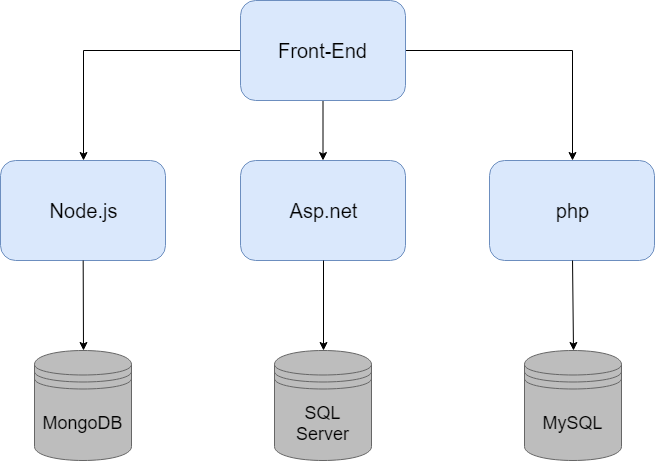
\includegraphics[width=\textwidth,keepaspectratio]{PizzaMicroservicii}
		      \caption{Arhitectur\u a cu microservicii pentru un site de pizzerie}
		      \label{fig:PizzaMicroservicii}
	      \end{figure}
	\item O aplica\c tie a c\u arei componente sunt distribuite este mai rezistent\u a, \^in sensul c\u a dac\u a un
	      serviciu este compromis, func\c tionalita\c tile care nu depind de acel serviciu vor continua s\u a func\c tioneze.
	      \^In cazul unei aplica\c tii clasice, tot sistemul va fi compromis din cauza unei singure componente.
	\item Cu un serviciu mare,monolitic, trebuie sa scal\u am totul \^imreun\u a.O parte mic\u a
	      a \^intregului nostru sistem, este constr\^ans\u a \^in performan\c t\u a, dar dac\u a
	      acest comportament este blocat \^intr-o aplica\c tie monolitic\u a gigant\u a, trebuie sa scal\u am totul \^impreun\u a
	      ca o bucat\u a \footcite{buildingMicroservices5}.Acest lucru se face deobicei folosind mai multe servere
	      \c si un server de tip load balancer care s\u a distribuie cererile c\u atre unul din acele servere pentru
	      a reduce munca depus\u a de un singur server o depune, astfel evit\^and supra\^incarcarea si cresc\^and performan\c ta.
	      \^In cazul arhitecturii cu microservicii, ajunge s\u a scalam doar acele servicii care au probleme de performan\c ta.
	\item Microserviciile ofer\u a \c si reutilizabiliate, ele pot fi utilizate de multiple aplica\c tii.
		  Daca dou\u a aplica\c tii au func\c tionalita\c ti similare, acestea nu trebuie implementate de dou\u a ori, aceast\u a func\c tionalitate
		  poate fi oferit\u a de un serviciu comun , folosit de ambele aplica\c tii.Uneori acest lucru este chiar necesar, dac\u a un produc\u ator de software
		  are mai multe aplica\c tii ce necesit\u a autentificare, este mult mai comod pentru utilizator s\u a aib\u a un singur cont cu care s\u a se autentifice in fiecare aplica\c tie 
		  \c si acest lucru este avantajos si pentru produc\u ator.
		  Microserviciile pot fi f\u acute \c si publice, pe baza unei chei de autentificare,pe care le pot folosi pentru aplica\c tiile lor,persoane in afara companiei produc\u atoare.
		  \^In prezent exist\u a multe servicii de meteorologie, gratuite sau contra cost, pe care le putem folosi \^in aplica\c tiile noastre.
\end{itemize}

Bine\^in\c teles arhitectura cu microservicii nu este o solu\c tie miraculoas\u a la toate problemele,
adat\u a cu aceste beneficii, ea vine \c si cu dezavantajele.Fiind un sistem distribuit toate
problemele acestor sisteme afecteaz\u a si microservicii.
O problem\u a este men\c tinerea leg\u aturii \^intre componentele aplica\c tiei.Un serviciu \^isi poate schimba 
adresa,poate deveni inactiv sau poate fi \^inlocuit.\^In aceste situa\c tii se va pierde func\c tionalitatea pe care acesta o 
ofer\u a.Pentru a remedia aceast\u a situa\c tie ar trebui sa schimb\u am adresele la care aplica\c tia se a\c steapt\u a sa 
gaseasc\u a serviciul respectiv, dup\u a care ar trebui sa to\c ti utilizatorii sa sa fac\u a un update la noua versiune.
Aceast\u a solu\c tie simpl\u a nu doar c\u a nu este convenabil\u a ,dar devine imposibil\u a dac\u a avem servicii care ruleaz\u a 
pe ma\c sini virtuale sau containere de docker care suntcreate dinamic \^in func\c tie de nevoie.
\section{Serviciu de \^inregistrare}
Solu\c tia pe care eu am implementat-o este un sistem de tip service registry.
Acesta este la baz\u a un serviciu web care face leg\u atura \^intre microservicii.Astfel aplica\c tia \c si serviciile trebuie 
s\u a cunoasc\u a doar serviciul de \^inregistrare si el se va furniza datele despre celelalte servicii necesare func\c tionarii aplica\c tiei. 
Serverul de \^ inregistrare ofer\u a trei opera\c tii de baza:
\begin{enumerate}
	\item \textbf{\^Inregistrarea}
	
			Serviciile se pot \^inregistra la server atunci c\^and \^i\c si \^incep func\c tionarea.
			\^In cazul \^in care serviciu folosit este facut de un alt produc\u ator care nu cunoa\c ste acest 
			mecanism sau nu este dispus s\u a \^il foloseasc\u a,exist\u a \c si posibilitatea ca administratorul 
			aplica\c tiei sa \^inregistreze serviciul respectiv manual prin intermediul intefer\c tei grafice.
	\item \textbf{De\^inregistrarea}

		  Serviciile au posibilitatea de a se de\^inregistra,acest lucru ar trebuie s\u a fie f\u acut la \^inchiderea 
		  serviciului.\^In cazul in care acestea devin inactive far\u a a se de\^inregistra, serverul le va de\^inregistra
		  automat.
	\item \textbf{C\u autarea}

		  Aplica\c tia \c si microserviciile pot c\u auta un serviciu \^inregistrat \^in server.
\end{enumerate}	
\section{Extensibilitate}
Extensibilitatea este o problem\u a permanent\u a \^in dezvoltarea de software.Un program poate \c si deobicei 
trebuie dezvoltat continuu.Serviciu de \^inregistrare, din cauza rolulului pe care \^il are, nu ar trebui oprit 
pentru actuazliz\u ari doar dac\u a acestea sunt absolut necesare \c si acest lucru trebuie s\u a se \^intample
c\^at mai rar posibil.\^In acest sens am implementat un mecanism de extensibilitate care nu necesit\u a oprirea
serverului.Aplica\c tia poate fi extins\u a prin add-inuri.Din acest motiv am expus un API pe care \^il pot folosi 
pentru dezvoltarea acestor add-inuri.Bine\^inteles, schimb\u arile mai importante nu pot fi f\u acute prin add-inuri
dar acestea reprezint\u a un mecanism suficient de bun pentru a ad\u auga func\c tionalit\u ati aplica\c tiei far\u a
a \^intrerupe fun\c tionarea serverului.Un alt avantaj al acestei abord\u ari const\u a \^in posibilitatea de 
ad\u augare de func\c tionalit\u ati la aplica\c tie de c\u atre utilizator. Acesta poate face un add-in 
folsind API-ul pe care \^il pun la dispozi\c tie.
Am ales s\u a ofer trei tipuri de add-inuri:
\begin{enumerate}
		\item \textbf{Add-In ac\c tiune}

			Acesta poate fi declan\c sat de c\u atre utilizator prin interfa\c ta grafic\u a.
		\item \textbf{Add-In periodic}

			Acest tip de add-in se execut\u a la un interval de timp.
		\item \textbf{Add-In pentru echilibrarea \^inc\u arc\u aturii}
		
			Acesta este un add-in special care con\c tine implementarea unui algoritm de echilibrare a \^inc\u arc\u aturii.
			\^In aplica\c tie poate exista un singur add-in pentru echilibrarea \^inc\u arc\u aturii.\^In cazul \^in care
			programul g\u ase\c ste mai multe astfel de add-inuri, este selectat aleator unul dintre ele.
\end{enumerate}

\section{Load Balancer}

Aplica\c tia mea, fiind un serviciu de \^inregistrare trebuie s\u a ia \^in calcul posibilitatea de a avea mai multe servicii
\^inregistrate cu acela\c si nume.Acest lucru poate p\u area c\u a ar trebui interzis \^ins\u a eu am ales s\u a accept \c si 
chiar s\u a \^incurajez aceast\u a situa\c tie.Cu acest scop am ad\u augat func\c tionalitatea de load balancing.
Load balanacing se traduce mot a mot \^in balansarea \^inc\u arc\u aturii \c si const\u a \^in distribu\c tia cererilor 
c\u atre un server \^intre mai multe servere identice.Cea mai direct\u a metod\u a de scalare a unui server este 
multiplicarea lui.Nu este suficient s\u a avem mai multe servere identice \c si s\u a las\u am utilizatorii s\u a
decid\u a ce server doresc s\u a foloseasc\u a,a\c sa c\u a folosim un load balancer care s\u a decid\u a care dintre
copiile serverului s\u a proceseze fiecare cerere \^in func\ tie de un algoritm.Doar serverul de balansare 
\c stie de existen\c ta serverelor pe care le are \^in grij\u a.
\begin{figure}[!htb]
	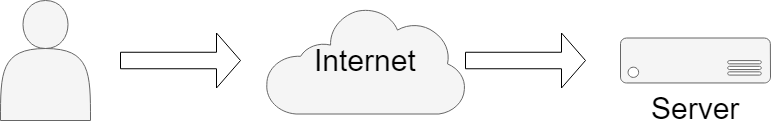
\includegraphics[width=\textwidth,keepaspectratio]{LoadNotBalanced}
	\caption{Accesarea unui server}
	\label{fig:notLoadBalanced}
\end{figure}
\begin{figure}[!htb]
	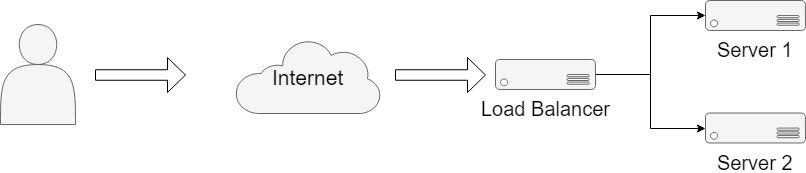
\includegraphics[width=\textwidth,keepaspectratio]{LoadBalanced}
	\caption{Accesarea unui server prin intermediul unei load balancer}
	\label{fig:loadBalanced}
\end{figure}

A\c s fi putut s\u a nu accept \^inregistrarea mai multor servicii cu acela\c si nume \c si echilibrarea \^inc\u arc\u aturii 
de munc\u a s\u a fie f\u acut\u a de fiecare serviciu \^in parte iar aplica\c tia mea s\u a \^inregistreze doar acest server
dar dac\u a rezolv \c si responsabilitatea de balansare elimin un punct de e\c sec.Dac\u a toate serviciile care au nevoie 
de scalare folosesc un load balancer atunci func\c tionarea lor depinde de acesta.Elimin\u and nevoia existen\c tei a \^inc\u a
unui risc cre\c ste siguran\c ta.

\chapter{Tehnologii}

\section{.NET Framework}
.NET este o platform\u a de dezvoltare a software-ului gratuit\u a pentru diverse sisteme de operare.
Platforma include o bibliotec\u a de mari dimensiunii numit\u a Framework Class Library \c si permite interoperabilitatea
a multor limbaje de programare.Programele scrise \^in .NET Framework ruleaz\u a \^intr-un mediu numit
Common Language Runtime(CLR), o ma\c sin\u a virtual\u a de aplica\c tie care ofer\u a servicii precum
securitatea, managementul memoriei \c si tratarea excep\c tiilor.Biblioteca de clase \c si CLR formeaz\u ua 
.NET Framework.\footcite{wikidotNet}

\section{C\#}

C\# este un limbaj de programare modern, orientat pe obiecte \c si puternic tipizat.C\# \^i\c si are r\u ada\u 1cinile
\^in familia de limbaje C \c si le este imediat familiar programatorilor C,C++ sau Java.C\# are multe caracteristici care
ajut\u a la construc\c tia palica\c tilor  robuste \c si durabile:
\begin{itemize}
	\item Garbage Collector-ul elibereaz\u a automat memoria ocupat\u a de obiectele care nu mai sunt folosite.
	\item Tratarea excep\c tilor ofer\u a o abordare structurat\u a \c si extensibil\u a pentru detectarea 
	erorilor \c si recuperare
	\item Designul puternic tipizat care face imposibil\u a existen\c ta variablilelor neini\c tializate,
		indec\c silor \^in afara limitelor \c sirurilor sau convertirea neverificat\u a a tipurilor.
\end{itemize}
C\# are un sistem de unificat de tipuri.Toate tipurile din limbaj,incluz\^and primitivele precum int,
mo\c stenesc dintr-o singur\u a r\u ad\u acin\u a tipul object.De aceea toate tipurile au un set de 
opera\c tii \c si valori de orice tip pot fi stocate,transportate \c si folosite pentru opera\c tii
\^intr-un mod consistent.

Pentru a se asigura faptul c\u a programele \c si bibliotecile C\# pot evolua \^in timp intr-o manier\u a compatibil\u a,
s-a pus accent pe versionare \^in designul limbajului.Multe limbaje de programare nu acord\u a suficient\u a aten\c tie
version\u arii \c si de aceea programele scrise \^in acele limbaje crap\u a nejustificat de frecvent atunci c\u and sunt
introduse veriuni noi ale bibliotecilor de care programul depinde.Aspecte din limbajul C\# care au fost influen\c tate 
de aceast\u a decizie includ modificatorii \verb1virtual1 \c si \verb1override1,regulile de supra\^inc\u arcare 
ale metodelor \c si suportul pentru declarare explicit\u a a interfe\c telor membre.\footcite{Hejlsberg:2003:CLS:861332}

\section{Asp.NET}

ASP.NET este un framework open-source pentru dezvoltarea web.A fost dezvoltat de Microsoft pentru a
le permite programatorilor s\u a creeze site-uri si servicii web dinamice.A fost introdus odat\u a cu
.NET framework 1.0 \c si ca urmare este construit pe CLR,ceea ce permite programatorilor sa utilizeze cod
scris in oricare limbaj suportat de platform\u a.La \^incpeuturile sale, dezvoltarea web site-urilor Asp.NET
era asociat\u a cu WebForms, care datorit\u a limit\u arilor sale a fost \^inlocuit e Asp.NET MVC. 

\subsection{Asp.NET MVC}
Asp.NET MVC reprezint\u a o alternativ\u a la WebForms pentru construc\c tia aplica\c tilor web \^in cadrul
platformei .NET.Asp.NET MVC are o abordare diferit\u a \^in ceea ce prive\c ste structura aplica\c tiei, folosind
arhitectura MVC.
Asp.NET MVC este mai aproape de protocoloul HTTP.spre deosebire de Web Forms care \^incearca s\u a ascunda 
natura far\u a stare a protocolului.Folosind arhitectura MVC \c si asociind o singur\u a cerere HTTP apel\u arii 
unei metode, experien\c ta dezvoltatorilor este mai naturala.

\^In timp ce Web Forms are o str\^ans\u a leg\u atur\u a \^intre logica aplica\c tiei \c si interfa\c ta grafic\u a,
Asp.NET MVC \^incurajeaz\u a un design \^in care interfa\c ta grafic\u a(view-ul) este separat\u a de codul
care o conduce(controller-ul).Atunci c\^and acest design este implementat corect, aplica\c tia devine mult mai u\c sor de men\c tinut
\c si dezvolatat.
De asemenea aceast\u a separare face componentele aplica\c tiei s\u a fie mult mai u\c sor de testat \^in isolare,
ceea ce faciliteaz\u a testarea automat\u a.

Una din componentele centrale ale paginilor Asp.NET MVC este motorul Razor.Acesta ofer\u a un mode concis
de a combina cod C\# \c si marcaj HTML pentru a crea pagini dinamic.Razor este esen\c tial pentru a afi\c sa 
utilizatorului rezultatul cererilor sale.Cu ajutorul Razor aceea\c si pagin\u a poate fi diferit\u a pentru 
fiecare utilizator.

\subsection{MVC pattern}
Model View Controller(MVC) este un \c sablon arhitectural care prezint\u a o solu\c tie pentru tratarea interfe\c tei grafice.
Arhitectura MVC este una dintre cele mai frecvent \^int\^alnite arhitecturi \^in dezvoltarea aplica\c tiilor web, deoarece
contribuie la scalabilitatea si extensibilitatea proiectelor.Separarea explicit\u a a responsabilit\u at\c tilor
cre\c ste pu\c tin complexitatea designului aplica\c tiei,dar beneficiile eclipseaz\u a efortul extra.\footcite{proAspNetMVC5Pattern}
MVC separ\u a aplica\c tia \^in trei componente:
\begin{enumerate}
	\item \textbf{Model}

		Componenta model corespunde logicii legate de date \c si prelucrarea lor.Asta poate \^insemna
		datele care sunt transferate \^intre componentele view \c si controller sau orice alte date care \c tin de
		logica aplica\c tiei.
	\item \textbf{View}

		Componenta View este folosit\u a pentru toat\u a logica ce \c tine de logica \^ interfe\c tei.
		\^In cazul aplica\c tilor web, view-ul este un \c sablon dupa care este generat codul HTML.
	\item \textbf{Controller}

		Componenta Controller func\c tioneaz\u a ca o interfa\c ta \^intre componentele view \c si model.
		Aceast\u a comonent\u a r\u aspunde inputului utilizatorului,comunic\u a cu modelul \c si decide 
		care view trebuie folosit ca rezultat al cererii.
\end{enumerate}
\begin{figure}[!htb]
	\includegraphics[width=\textwidth,keepaspectratio]{MVCPattern}
	\caption{Arhitectur\u a MVC}
	\label{fig:MVCPattern}
\end{figure}
\subsection{Asp.NET WebApi}
Un web api este o interfa\c t\u a programatic\u a la un sistem care este accesat\u a prin metode standard HTTP.
Un web api poate fi accesat de o varietate larg\u a de clienti HTTP, incluz\^and browser \c si dispozitive mobile \footcite{evolvableWebApi}.

Asp.net MVC este construit cu scopul de a face website-uri.Acest lucru este evident din func\c tionarea acestui framework,
r\u aspunde la cereri primite din browser \c si returneaz\u a HTML.Cu toate acestea Asp.NET MVC permite un control minu\c tios
asupra r\u aspunsului dat,\c si MVC este util \^in formarea unui web api.Dezvoltatorii asp.net au realizat c\u a puteau folosi
acest framework pentru dezvoltarea de servicii web \c si aceasta improviza\c tie era preferabil\u a alternativelor.\footcite{proAspNetMVC5Asp}

Din acest motiv,odat\u a cu Asp.NET MVC 4,a fost introdus si Asp.net Web Api,un framework care ofer\u a 
stilul de lucru din Asp.NET MVC adaptat pentru a scrie servicii web.

\section{JavaScript}
JavaScript este un limbaj de programare interpretat cu capabilit\u a\c ti de orientare pe obiect.
JavaScript este sintactic similar cu C,Java \c si C\#,\^inc\u a similarit\u a\c tile se termina la sintax\u a.
JavaScript este un limbaj slab tipizat,ceea ce \^inseamn\u a c\u a variabilele nu au un tip specificat.
Obiectele asociaz\u a nume de propriet\u a\c ti unor valori arbitrare \c si se aseam\u n\u a mai mult
cu hashtable-urile din C\# dec\^at cu obiectele.Mecanismul de mo\c stenire din JavaScript este bazat pe
prototip \c si nu se aseam\u an\u a cu cea din C++ sau c\#.
Tipurile primive din JavaScript sunt numere,stringuri \c si valori booleene dar limbajul include \c si
date,\c siruri \c si expresii regulate.\footcite{Flanagan:2011:JDG:2029041}

Motivul principal pentru care am les s\u a folosesc acest limbaj \^in proiectul meu este faptul c\u a 
JavaScript este limbajul cunoscut de toate browser-ele \c si \^in acel context este extins cu obiecte care
permit interac\c tiunea cu utilizatorul, alterarea con\c tinutului paginii care 
este \^inc\u arcat\u a \^in browser \c si  controlul browser-ului.Aceast\u a versiune a limbajului
este numit\u a \c si JavaScript \verb1client-side1 pentru a sublinia faptul c\u a scripturile func\c tioneaz\u a
\^in browser-ul clientului \c si nu pe server.

De\c si JavaScript este utilizat predominant \^in dezvoltarea paginilor web,datorit\u a popularit\u a\c tii 
acestuia, s-au dezvoltat numeroase 
framework-uri dedicate acestui limbaj care permit dezvoltarea pe diferite platforme.
Cu Node.js JavaScript poate fi folosit pentru a face servere web.Electron.js permite ca JavaScript
s\u a fie folosit pentru aplica\c tii desktop cross-platform.JavaScript poate fi folosit \c si pentru
aplica\c tii pentru dispozitivele mobile prin intermediul frameworkurilor Ionic sau React.js. 

\section{HTML}

Hypertext Markup Language(HTML) este limbajul de marcaj standard pentru creearea paginilor web \c si aplica\c tiilor web.\footcite{wikiHTML}\^Impreun\u a cu 
CSS \c si JavaScript formeaz\u a cele trei limbaje esen\c tiale care definesc interfa\c ta grafic\u a a unei aplica\c tii web.
Navigatoarele web primesc documente HTML de la un server \c si pe baza acestuia afi\c seaz\u a o pagin\u a web.HTML descrie 
structura semantic\u a a unei pagini.

Elementele HTML sunt blocuri de construc\c tie ale paginilor HTML.Folosind HTML se pot introduce \^in pagini obiecte precum imaginile
sau form interactive se pot introduce \^intr-o pagin\u a web.De asemenea,HTML permite crearea unor documente structurate, denot\^and
structural semantice pentru text precum paragrafe, liste, linkuri, gilimele \c si altele.Elementele HTML sunt delimitate de taguri
scrise folosind paranteze unghiulare.Exist\u a taguri care introduc direct elemente, precum tagul <img/>.Pe de alt\u a
pare exist\u a \c si taguri care dau informa\c tii despre subelementele acestora, precum tagul <strong>.
Navigatoarele nu afi\c seaz\u a direct documentele HTML, ci stiu s\u a le interpreteze.Despre elementele 
HTML se pot da informa\c tii suplimentare prin atributele acestora.Majoritatea atributelor sunt perechi
de tip cheie valoare separate prin semnul "=".De asemenea valoarea atributelor trebuie specificat\u a \^intre ghilimele.
Atributele se g\u asesc mereu \^in tagul de \^inceput al elementelor HTML.

\section{CSS}

Cascading Style Sheets(CSS) este un limbaj de stil folosite pentru descrierea prezent\u arii documentelor scrise \^in HTML.
CSS a fost conceput pentru a permite separarea \^intre prezentare \c si con\c tinut, incluz\^and forme,culori \c si fonturi.
Aceast\u a separare poate \^imbun\u at\u a\c ti accesibilitatea con\c tinutului.De asemenea separarea permite mai mult\u a 
flexibilitate \c si control \^in specificarea caracteristicilor prezent\u arii.Un alt beneficiu pe care \^il aduce CSS este 
faptul c\u a mai multe pagini web pot folosi acelea\c si stiluri, dintr-un fi\c sier .css, ceea ce reduce complexitatea
\c si repetabilitatea.Mai mult,folosind acela\c si fi\c ier css putem  da un aspect similar paginilor care fac parte din 
aceea\c si aplica\c tie,cree\^and o unitate \^inte acestea.Numele cascading din CSS provine de la metoda pe prioritizare 
a stilurilor care afecteaz\u a un element.CSS folose\c ste prioritate de tip cascade pentru a determina regula de stil aplicat\u a 
unui element atunci c\^and acesta este afectat de mai mult reguli.CSS alege regula care va fi folosit\u a parcurg\^and \^in cascad\u a toate
regulile aplicate elementului pornind de la cea mai general\u a p\^an\u a la cea mai specific\u a. 

\^Inainte de CSS,HTML era folosit \c si pentru partea prezentare, motiv pentru care au ap\u arut foarte multe taguri HTML
cu rol de prezentare.HTML a fost conceput pentru a avea un rol structural \^in pagin\u a dar a devenit din ce \^in ce mai 
aglomerat cu taguri de prezentare\footcite{cssDef}.Aceast\u a poluare a limbajului a fost sesizat\u a \c si de c\u atre World Wide Web Consortium (W3C)
care au c\u autat o solu\c tie la problem\u a.Solu\c tia propus\u a de W3C a fost CSS care a devenit o recomandare cu aceea\c si greutate
ca HTML.De atunci CSS a evoluat odat\u a cu dezvoltarea web, p\^an\u a la starea \^in care se afl\u a ast\u azi.

\section{Entity Framework}
P\^ana la .NET 3.5,programatorii obi\c snuiau sa foloseasc\u a ADO.NET pentru a alva sau prelua date din 
baza de date.Trebuiau deschise conexiuni, create DataSeturi pentru a citi sau scrie date care mai apoi trebuiau 
convertite \^in obiect sau invers.Acesta era un proces greoi \c si predispus la erori.Odat\u a cu .NET 3.5
Microsoft a introdus EntityFramework cu scopul de automatiza lucrul cu baze date.

EntityFramework este un ORM(Object Relational Mapper) open-source creat de Microsoft pentru platforma .NET.
Framework-ul premite programatorilor s\u a utilizeze datele prin intermediul  unor obiecte specifice domeniului
far\u a a se concentra pe tabelele \c si coloanele \^in care datele sunt stocate.Acest lucru permite dezvoltatorilor 
s\u a lucreze la un nivel mai \^inalt de abstractizare atunci c\^ and lucreaz\u a cu date persistente.

EntityFramework ofer\u a dou\u a modalit\u a\c ti de lucru:
\begin{itemize}
	\item \textbf{Code First}

		Aceast\u a abordare necesit\u a ca programatorul s\u ascrie clasele corespunz\u atoare datelor care trebuie s\u a persiste \^in baza de date \c si 
		o clasa speciala numit\u a context.Pe baza acestora el poate genera o baz\u a de date.Baza de date generat\u a
		se poate actualiza prin migra\c tii.Migra\c tie ofer\u a un mode incremental de a aplica schimb\u ari unei baze
		de date generate cu EntityFramework pentru a o sincroniza pe aceasta cu clasele care consitiuie modelul. O migra\c tie
		con\c tine toate scimb\u arile modelului care trebuie reflectate \^in baza de date de la ultima actualizare.
		\^Impreun\u a toate migra\c tile formeaz\u a istoria bazei de date.

	\item \textbf{Database First}

		\^In aceast\u a abordare EntityFramework creaz\u a clasele model be baza unei baze de date deja existente printr-un proces numit
		scaffolding.Termenul scaffolding provine din domeniul construc\c tiilor \c si \^inseamna procesul de montare a schelelor unei cl\u adiri.
		Precum schelele fac posibil\u a construc\c tia unei cl\u adiri, a\c sa modelul face posibil\u a prelucrarea datelor din baza de date.
		Aceast\u a este abordarea pe care am decis s\u a o folosesc \^in realizarea acestui proiect.
	\item \textbf{Model First}
		Abordarea Model first presupune creare entit\u a\c tilor \c si rela\c tilor dintre acestea \^intr-o schem\u a,utiliz\^and un designer grafic.
		Pe baza schemei sunt generate clasele ce constituie modelul \c si baza de date.
\end{itemize} 
Din experien\c ta mea cu variantele prezentate, am ajus s\u a prefer varianta database first, deoarece consider c\u a astfel am mai mult control
asupra datelor \c si opera\c tiilor.

\section{Microsoft SQL Server}
Microsoft SQL Server este un sitem de management al bazelor de date rela\c tionale,care sus\c tine o varietate
larg\u a de aplica\c tii.Precum alte sisteme de management al bazelor de date relaz\c tionale,SQL Server
este construit peste SQL, un limbaj standardizat pe care administratorii de baze de date \c si profesioni\c stii IT
\^il folosesc pentru a manageria baze de date \c si pentru a interoga dateele pe care acestea le con\c tin.
SQL Server este legat de Transact-SQL, o Implementare a SQL de la Microsoft care adaug\u a un set de extensii 
de programare limbajului standard.
Componenta central\u a a SQL Server este motorul bazei de data,care controleaz\u a stocarea datelor, procesarea lor
\c si securitatea.Acesta include un motor rela\c tional care proceseaz\u a comenzi \c si interog\u ari \c si 
un motor de stocare ce manageriaz\u a fi\c sierele, tabele, paginile, indec\c si, buffer-ele de date \c si tranzac\c tile.
Procedurile stocate, trigger-ele,view-urile \c si celelalte obiecte ale bazei de date sunt deasemenea create \c si executate 
de motorul bazei de date.\footcite{sqlServer}
Mai jos dec\^at motorul bezei de date se alfa sistemul de operare al SQL Server(SQLOS) care se ocup\u a
de opera\c tii de nivel sc\u azut precum managementul memoriei \c si intr\u arilor \c si ie\c sirilor, programarea joburilor 
\c si blocarea datelor pentru a evita conflictele la actualizare.Deasupra motorului bazei de date se afla un strat de re\c tea,
care folose\c ste protocolul Tabular Data Stream al Microsoft pentru a facilita interac\c tiunile de tip cerere \c si r\u aspuns
cu serverul.

\chapter{Implementare}

\section{Arhitectura}

Aplica\c tia este construit\u a urm\^and o arhitectur\u a pe straturi.
\^in arhitectura pe straturi componentele apicla\c tiei sunt organizate \^in starturi orizontale,
fiecare \^indeplinind un rol specific \^in cadrul aplica\c tiei.Fiecare strat este o abstractizare 
a \^in jurul cerin\t elor aplica\c tiei.Una din tr\u as\u aturile definitorii ale acestei arhitecturi
este separarea responsabilit\u a\c tilor.Componentele unui strat al aplica\c tiei se procup\u a doar 
cu logica specific\u a stratului \c si nu se intersecteaz\u a cu logica altor straturi.
Nu exist\u a un num\u ar impus de straturi, \^in unele cazuri anumite straturi pot lipsi sau pot 
ap\u area noi straturi.

Serviciul meu de \^inregistrare este compus din 4 straturi, \c si anume:
\begin{enumerate}
	\item Un strat de stocare al datelor
	\item Un strat de accesare a date
	\item Un strat de logic\u a de business
	\item Un strat de prezentare
\end{enumerate}

\subsection{Stratul de stocare a datelor}

Acest strat const\u a \^in baza de date.
Pentru c\u a am folosit EntityFramework \^in modul Database First am \^inceput proiectul cu arhitecturii
bazei de date.Dac\u a \^in viitor vor ap\u area probleme de performan\c t\u a voi putea optimiza accesarea datelor
scriind prorpile proceduri stocate mai eficiente dec\^at cele generate de EntityFramework pe baza codului.
Pentru a putea interac\c tiona cu aplica\c tia prin interfa\c ta grafic\u a \^intr-un mod securizat este nevoie 
de un sitem de autentificare deci trebuie stocate date despre utilizator.Pentru autentificare fiecare utilizator
trebuie s\u a poate fi indentificat unic \c si din motive de securitate evindente el are nevoie de o parol\u a
a c\u arei valoare hash este stocat\u a \^in baza de date.Pentru partea de autorizare este nevoie ca fiec\u arui 
utilizator s\u a \^ii fie asociat unul sau mai multe roluri.\^In func\c tie de rolul unui utilizator,aplica\c tia decide
dac\u a acestui \^ii este permis accesul la o anumit\u a func\c tionalitate.Administratorul serviciului
va avea toate rolurile \c si ca urmare va avea acces nerestric\c tionat.\^In prezent  mai exist\u a un singur alt tip
de utilizator, al c\u arui singur nu rol \^ii permite s\u a fac\u a modific\u ari pe server.Acest rol este inte\c tionat
pentru programatorii care lucreaz\u a cu unul sau mai multe din serviciile \^inregistrate \c si le pune la dispozi\c tie 
informa\c tii legate de starea serviciilor.Sistemul de roluri este g\^andit \^in a\c sa fel \^inc\^at  s\u a fi u\c sor 
de ad\u augat \c si integrat un rol nou.Introducerea unui rol nou nu va afecta cu nimic rolurile existente \c si nici
utilizatorii existen\c ti.Rolurile pot fi asgnate \c si utilizatorilor vechi d\^andule astfel noi permisiuni.


Pentru ca utilizatorii s\u a aib\u a mai multe informa\c tii, am implementat un mecanism de mesagerie.Acesta nu este 
inten\c tionat ca un mijloc de comunicare \^intre utilizatori, ci este un mod ca ei s\u a fie informa\c ti de sistem.
Deoarece add-inurile au acces la mesaje, nu exist\u a o regul\u a cu privire trebuie s\u a cont\c tin\u a un mesaj.
Acestea pot con\c tine orice de la inform\u ari cu privire la servicii care nu au mai fost folosite de mult, p\^an\u a
la mesaje de \^in\^ampinare a unui nou utilizator.Dup\u a cum se vede \c si in Figura \ref{fig:DbUser}, un mesaj 
are un destinatar \c si un expiditor.Acest lucru poate fi folosit dac\u a pe viitor utilizatorii vor avea nevoie s\u a
 \^i\c si poat\u a trimite mesaje unul altuia, dar \^in prezen expeditorii mesajelor sunt add-inurile.
 Fiecare add-in are asociat un utilizator special f\u a\u a nici un rol.


\begin{figure}
	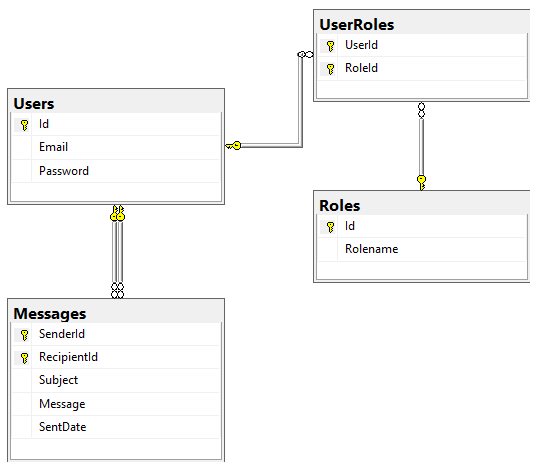
\includegraphics[width=\textwidth,keepaspectratio]{DbDiagramUsers}
	\caption{Diagrama rela\c tiilor utilizatorului}
	\label{fig:DbUser}
\end{figure}

Pentru un serviciu de \^integistrare cele mai importante date sunt cele referitoare la serviciile \^inregistrate.
Un serviciu este identificat prin numele de cluster \c si numele de aplica\c tie.Cluster-ul define\c ste grupul
din care face parte un serviciu.Nu exist\u a o restric\c tie de unicitate pentru combina\c tia nume de cluster \c si
nume de aplica\c tie, deoarece func\c tia de load balancing se func\c tioneaz\u a atunci c\^and exist\u a mai multe 
servere identice. Pentru a putea fi folosit,un serviciu are nevoie \c si de un URL.URL-ul trebuie s\u a fie unic \^in 
cadrul unui cluster.Nu are sens ca acela\c si serviciu s\u a fie \^inregistrat de dou\u a ori,\^ins\u a nu ar trebui 
s\u a fie oprit din a fi folosit \^in mai multe clustere, astfel URL-ul nu trebuie s\u a fie unic, ci combina\c tia 
cluster,URL. Dup\u a cum se poate observa \c si \^in figura \ref{fig:DbServices}, am ad\u augat un tabel destinat
monitoriz\u arii acces\u arii serviciilor.\^In etapa ini\c tial\u a a proiectului acest tabel era \^inlocuit de 
c\u atre o coloan\u a \^in tabelul Services care con\c tinea data ultimei acces\u ari a serviciului.De\c si 
data ultimei acces\u ari este o informa\c tie important\u a, nu este suficient\u a.Stoc\^and fiecare accesare 
pot realiza statistici relevante pentru utilizatori.

\begin{figure}[!ht]
	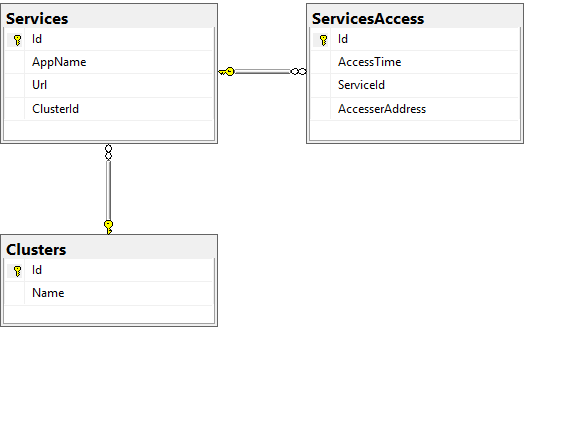
\includegraphics[width=\textwidth,keepaspectratio]{DbDiagramServices}
	\caption{Diagrama serviciilor}
	\label{fig:DbServices}
\end{figure}


\pagebreak

\subsection{Stratul de accesare a datelor}

Stratul de accesare a datelor const\u a \^intr-un proiect separat ce con\c tine interfe\c te \c si clase 
 care au responsabilitatea de a prelua sau prelucra datele din baza de date.Aceast\u a separare aduce numeroase
 beneficii:
 \begin{itemize}
	 \item Am eliminat duplicarea codului de acces la date.
	 \item Separearea responsabilit\u a\c tiilor cre\c ste mentenabilitatea \c si citibilitatea codului
	 \item Datorit\u a decupl\u arii am f\u acut codul testabil \^in izolare.Un alt avantaj
	 \item Am decuplat aplica\c tia de framework-ul de persisten\c t\u a, astfel este mai u\c soar\u a schimbarea
	 	acestuia dac\u a \^in viitor va ap\u area nevoia. 
 \end{itemize}
 
Accesarea datelor se face prin interfe\c te, a c\u aror implementare este ob\c tinut\u a prin injectare de dependen\c te
Am definit c\^ate o interfa\c t\u a pentru fiecare entitate persistent\u a major\u a.

Interfa\c ta IUserRepository con\c tine 
metode pentru accesarea datelor despre utilizatori, sau trimiterea mesajelor c\u atre utilizatori.Un mesaj poate fi trimis c\u atre 
un singur utilizator sau c\u atre to\c ti utilizatorii care \^indeplinesc o anumit\u a condi\c tie.Pentru a stabili o condi\c tie 
de trimitere c\u atre mai mul\c ti utilizator am folosit un delegat pentru o metod\u a ce prime\c ste ca parametru un obiect de tip 
User \c si returneaz\u a un r\u aspuns boolean.

Interfa\c ta IClusterRepository define\c ste metodele clasice ale unui repository, \c si anume opera\c tiile CRUD \c si o metod\u a de
filtrare folosind un delegat.

Interfa\c ta IServicesRepository este probabil cea mai important\u a, deoarce corespunde fun\c tionalit\u atii principale ale aplica\c tiei.
Este evident c\u a aceast\u a trebuie s\u a aib\u a metode pentru \^inregistrarea,de\^inregistrarea \c si g\u asirea serviciilor.
De asemenea este nevoie \c si de o metod\u a pentru a ob\c tine toate serviciile, astfel \^inc\^at acestea s\u a poat\u a fi 
afi\c sate \^in interfa\c ta grafic\u a.Tot pentru partea vizual\u a a aplica\c tiei am avut nevoie \c si de un mod de a aduce 
din baza de date toate acces\u arile unui serviciu dintr-un interval e timp.Pe baza dateloe de acces pot realiza staticstici referiotare
la accesul la servicii.

Tot \^in stratul de accesare a datelor se afl\u a \c si Interfa\c ta ILoadBalancer\ref{lst:ILoadBalancer}.Clasa ServicesRepository care implementeaz\u a
interfa\c ta IServicesRepository se folose\c ste de un obiect ce implementeaz\u a interfe\c ta ILoadBalancer, ca o strategie.
Strategia este un \c sablon de proiectare comportamental care permite schimbarea algoritmului \^in timpul rul\u arii aplia\c tiei.
Acest lucru se face trimi\c t\^and un obiect ce implementeaz\u a ILoadBalancer prin constructorul clasei ServicesRepository.
Pentru interfa\c ta ILoadBalancer am f\u acut \c si o implementare implicit\u a, care este folosit\u a \^in cazul \^in care nu exist\u a o implementare sub form\u a de 
add-in.Acest\u a implementare va returna url-ul serverului care a fost folosit \^in urma cu cea mai \^indelungat\u a perioad\u a \c si se potrive\c ste 
serviciului c\u autat.Parametrii clusterName \c si appName ai metodei GetService sunt folosi\c ti pentru a identifica serviciul,
iar  parametrul ipAddress reprezint\u a adresa ip a celui care solicitat serviciul respectiv.Adresa ip trebuie stocat\u a odat\u a
cu data acces\u arii serviciului.

\begin{lstlisting}[caption={Interfa\c ta ILoadBalancer},label={lst:ILoadBalancer}, breaklines]	
    /// <summary>
    ///     Strategy for load balancing algorithm
    /// </summary>
    public interface ILoadBalancer
    {
        /// <summary>
        ///  Get a service using a load balancing algortihm
        /// </summary>
        /// <param name="clusterName"></param>
        /// <param name="appName"></param>
        /// <param name="ipAddress"></param>
        /// <returns></returns>
        Service GetService(string clusterName, string appName, string ipAddress);
    }
\end{lstlisting}

\pagebreak

\subsection{Startul de logic\u a de business}

Startul  de logic\u a de business con\c tine 2 proiect.Un proiect dedicat Add-inurilot \c si unul dedicat utiliz\u arii 
datelor venite din stratul de acces al datelor.\^In acest proiect se g\u asesc trei interfe\c te \c si implement\u ariile lor.
Interfe\c telor IServicesRepository,IUserRepository \c si IClusterRepository  din stratul precedent,le corespunde o 
interfa\c t\u a \^in acest strat.Pentru IServicesRepository exist\u a IServicesManager,pentru IClusterRepository exist\u a 
IClusterManager \c si pentru IUserRepository exist\u a IUserManager.Implement\u arile interfe\c telor de tip manager se folosesc
de obiecte de ce implementeaz\u a interfe\c tele repository corespunz\u atoare pentru a accesa datele.Aceste obiecte sunt 
furnizate prin procedeul inject\u arii dependen\c telor.Astfel ServicesManager care  implementeaz\u a interfa\c ta 
IServicesManager, prime\c te o implementare a IServicesRepository prin care realizeaz\u a accesarea \c si prelucrarea datelor.
Folosind interfe\c te, managerii nu depind de modul \^in care datele sunt stocate.Metodele managerilor au rolul de a face 
valid\u arii asupra parametriilor cu are sunt apelate pentru a preveni caut\u ari inutile printre datele stocate sau
inserarea unor date are ar putea afeta consisten\c ta datelor stocate.Cu toate aceastea managerii nu se limiteaz\u a 
la valid\u ari,clasele repository doar aduc datele,tot resutl logicii se petrce \^in manageri.Se poate spune c\u a un repository
este o unealt\u a care \^ii d\u a acces la date unui manager.

\^In cel\u alalt proiect din acest strat se afl\u a logica ce guverneaz\u a add-inurile.Ca un add-in 
s\u a fie \^inc\u arcat \^in aplica\c tie acesta trebuie s\u a fie fac\u t cunoscut aplica\c tiei.
Acest lucru se face printr-un fisier de tip *.sAddIn care define\c ste add-inul.Fi\c sierele *.sAddIn sunt fi\c siere
\^in format JSON care conc\c tin informa\c tii despre addIn.Dup\u a  cum se vede \^in \ref{lst:addInDef}, defini\c tia 
unui add-in trebuie s\u a con\c tin\u a numele add-inului,o scurt\u a descriere,tipul de add-in, intervalul la care 
acesta trebuie executat \c si calea c\u atre add-in.Intervalul este exprimat \^in ore \c si este luat \^in considerare 
doar pentru add-inurile periodice.
loca\c tia de pe disc a add-inului. 
\begin{lstlisting}[caption={Defini\c tie a unui AddIn},label={lst:addInDef},breaklines]
{
	"Name":"UnusedServiceNotifier",
	"ShortDescription":"Sends a notification to the administrators regarding unused services",
	"Type":"Periodic",
	"RunInterval":4,
	"Path":"/AddIns/Periodic/USN.dll"
}
\end{lstlisting}
Pe l\^ang\u a un fis\c ier \^il define\c ste, pentru a putea fi executat un add-in trebuie s\u a con\c tin\u a o clas\u a 
ce implementeaz\u a Interfa\c ta IAddin.Aceast\u a clas\u a este punctul de intrare \^in add-in.

\^In prezent din punct de vedere al limbajului de programare folosit, add-inurile se \^impart in dou\u a categorii, \c si
anume add-inuri scrise \^in C\# \c si add-inuri scrise \^in CSScript.Add-inurile C\# sunt sub form\u a de dll iar 
cele scris \^in CSScript sunt fi\c siere text cu extensia .csscript.Problema \^in aceast\u a situa\c tie este c\u a 
ambele tipuri de add-inuri trebuie tratate la fel \^ins\u a este evident c\u a execu\c tia acestor se face diferit.
Bilbiotecile trebuie \^inc\u arcate \^in aplica\c tie apoi prin mecanismul reflection trebuie g\u asit\u a 
clasa ce implementeaz\u a interfa\c ta IAddin \c si apoi exceutat\u a metoda Run a acesteia.
Pe de alt\u a parte fi\c siere CSSript sunt fi\c siere text \c si acestea trebuie interpretate de un interpretor CSScript.
Interpretorul caut\u a punctul de intrare \^in add-in \c si apoi execut\u a metoda Run.Cu siguran\c t\u a nu pot \^In ciuda diferen\c tei dintre 
cele dou\u a tipuri de add-inuri, ele trebuie tratate similar de c\u atre aplica\c tie.
Am rezolvat o parte din problem\u a definind o interfa\c t\u a IAddInRunner care s\u a se ocupe de lansarea \^in execu\c tie 
a extensilor.Prin intermediul acesteia, procesul de ad\a ugare al unui nou tip de add-in se reduce la crearea unei noi
implement\u ari a interfe\c tei, potrivit\u a pentru tipul dorit.Nu doar c\u a am fac\u at posibil\u a implementarea add-inurilor
 sub forma de bibliotec\u a cu leg\u atur\u a dinamic\u a \c si sub form\u a de scrip CSScript, dar am \c si preg\u atit
 aplica\c tia pentru dezvoltare viitoare.Singur a problem\u a r\u amas\u a este faptul c\u a aplca\c tia are nevoie de un mod
 de a \c sti ce fel de add-inuri s\u a foloseasc\u a.Decizia cu privire la tipul de add-in se face dintr-un fi\c sier de 
 configurare.O posibil\u a solu\c tie ar fi ca la oric\^and este nevoie ca aplica\c tia s\u a stie ce fel de extensii trebuie 
 s\u a foloseas\u a, aceast\u a s\u a fac\u a o verificare.Aceast\u a abordare nu doar c\u a va polua codul cu interog\u ari
 \c si va cauza duplicare de cod, dar este \c si foarte greu de \^intre\c tinut \c si dezvoltat.Solu\c tia mea a fost
s\u a folosesc o implementare de tip abstract factory \ref{fig:IAddInRunnerFactory}.Abstract Factory este un \c sablon de proiectare care ofer\u a 
o interfa\c t\u a pentru creearea unei familii de obiecte \^inrudite sau dependente f\u ar\u a specificarea claselor
lor concrete.\footcite{Freeman:2004:HFD:1076324} 

\begin{figure}[!ht]
	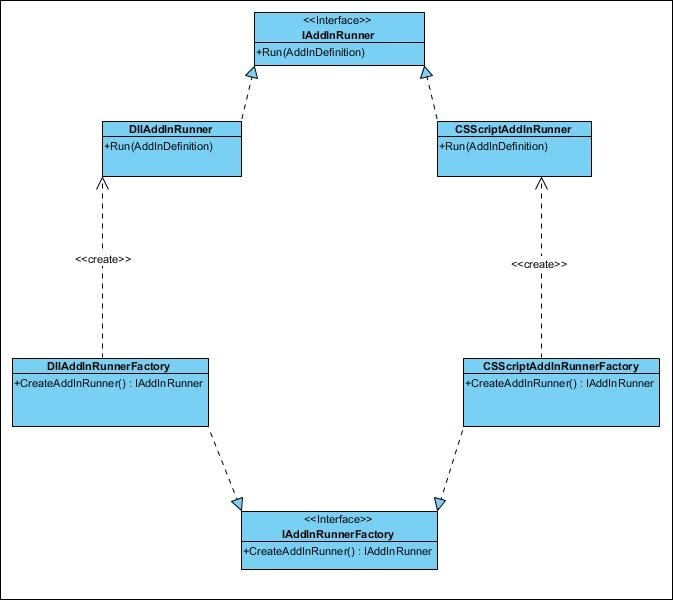
\includegraphics[width=\textwidth,keepaspectratio]{IAddInRunnerFactory}
	\label{fig:IAddInRunnerFactory}
\end{figure}

\^In func\c tie de tipul de addIn specificat \^in fi\c sierul de configurare al serverului,se va alege care implementare a 
interfe\c tei IAddInRunnerFactory va fi folosit\u a de aplica\c tie.Implementarea aleas\u a va fi folosit\u a \^in \^intreaga
aplica\c tie  \c si astfel cu o singur\u a verificare programul va folosi tipul de add-inuri dorit.

Exist\u a situa\c tii \^in care un add-in devine irelevant sau nedorit de utilizator, din acest motiv,Add-Inurile trebuie 
s\u a poat\u a fi \c sterse de utilizator.Pentru a ad\u auga aceast\u a func\c tionalitate, am creat \c si implementat o
 interfa\c ta dedicat\u a st\u arii de pe disc a add-inurilor.Aceast\u a interfa\c t\u a poate reg\u asi add-inurile de pe disc
 \c si le poate \c sterge.

 Dup\u a cum am men\c tionat mai devreme exist\u a un tip de add-inuri care sunt executate periodic.Fiecare add-in de acest tip 
 are un alt interval orar la care trebuie executat.Cu scopul de a planifica \c si lansa \^in execu\c tie aceste add-inuri am f\u a cut
 clasa AddInScheduler.AddInScheduler opereaz\u a \^intr-un fir de execu\c tie separat datorit\u a naturii asincrone a acestuia.
  AddInScheduler se ocup\u a de lansarea \^in execu\c tie a tuturor add-inurilor ce trebuie executate periodic.
 Clasa ofer\u aposibilitatea ad\u aug\u arii unui add-in nou oric\^and \c si la dispari\c tia unui add-in de pe disc, AddInScheduler
 \^il va scoate automat din lista de excu\c tie.Din nou intervine problema lans\u arii \^in execu\c tie a add-inurilor,
 dar de data aceasta este \^in cadrul AddInScheduler.De\c si \^in cazul unei implement\u ari naive, execu\c tia add-inurilor
 de c\u atre AddInScheduler ar putea p\u area o problem\u a,defapt execu\c tia nu este treaba acestei clase.
 Tot ce trebuie s\u a fac\u a clasa AddInScheduler este s\u a foloseasc\u a o implementare a interfe\c tei IAddInRunner 
 care la r\^andul ei s\u a se ocupe de execu\c tia add-inurilor.\c Si dup\u a cum am stabilit anterior, AddInScheduler
 va ob\c tine o implementare corect\u a a IAddInRunner printr-un factory. 

\subsection{Stratul de prezentare}

La acest strat aplica\c tia se bifurc\u a form\^and dou\u a servere.Primul server este serviciul de \^inregistrare
care este component\u a principal\u a a proiectului meu.Acesta este un server de tip Web Api astfel interfa\c ta grafic\u a
\^int\^alnit\u a \^in mode obi\c snuit \^in stratul de prezentare este \^inlocuit\u a de o interfa\c t\u a de comunicare
cu serverul prin intermediul HTTP.Stratul de prezentare din webapi are o arhitectur\u a MVC \^in care lipse\c ste partea
de View.

Al doilea server este interfa\c ta grafic\u a a aplica\c tiei \c si permite administrarea aplica\c tiei.\^In cazul 
acestui server stratul de prezentare se reg\u ase\c ste \^in sensul clasic.Arhitectura stratului este MVC complet spre
deosebire de cazul anterior.

Toate starturile precedente sunt comune \^in cele dou\u a servere.
Separarea aplica\c tiei ini\c tiale \^in dou\u a servere distincte nu doar reduce munca fiec\u arui server,
dar \c si faciliteaz\u a dezvoltarea.

Inte\c tia implement\u arii pe straturi este o cuplare mai slab\u a \^intre modulele aplica\c tiei.Acest lucru este 
realizat prin folosirea interfe\c telor \^in locul implement\u arilor concrete \c si prin injectarea dependen\c telor.
\^In Asp.NET MVC \c si Web Api toate cererile utilizatorilor sunt trimise c\u atre un Controller care se ocup\u a de
r\u astpunsul la acestea.Controller-ele sunt instan\c tiate de c\u atre framework ceea ce m\u a \^impideic\u a s\u a 
fac o injectare de dependen\c te clasic\u a.Asta nu \^inesamn\u a c\u a trebuie s\u a deteriorez  arhitectura, ci 
trebuie s\u a fac injectarea dependen\c telor printr-un alt mod.Abordarea alternativ\u a este oferit\u a de c\u atre 
Autofac.Autofac este un container pentru inversarea controlului.Cu autofac pot \^inregistra \^intr-un container 
implement\u arile interfe\c telor de care am nevoie \c si atunci c\^and va fi nevoie de o implementare, se va folosi tipul
\^inregistrat \^in container.De exemplu,c\^and se va crea o instan\c t\u a a clasei AccountController, care necesit\u a 
implement\u area interfe\c tei IUserManger,acesta va primi o nou\u a instan\c t\u a a clasei UserManager \c si pentru ca 
aceasta necesit\u a o implementare a IUserRepository, \c si UserManager va primi implementarea IUserRepository \^inregistrat\u a
\^in container.Cu autofac pot \^inregistra \c si tipuri \^in timpul rul\u arii, cum am f\u acut \^in cazul interfe\c tei 
ILoadBalancer, a c\u arei implementare se caut\u a \^intr-un add-in.

 

\section{Autentificarea \c si autorizarea}

\^In asp.net exist\u a un framework numit IdentityModel care se ocup\u a de o mare parte din autentificarea \c si autorizarea
utilizatorilor.Acesta se integreaz\u a bine cu framework-ul ASP.NET MVC \c si este suficient pentru securitatea majorit\u atii 
aplica\c tiilor.IdentityModel este de asemenea u\c sor de folosit \c si cu un efort minim o aplica\c tie poate avea partea de 
autentificare \c si autorizare func\c tional\u a.Din aceste motive este foarte comun \^in aplica\c tiile ASP.NET.

Cu toate aceste beneficii pe care le aduce, IdentityModel este un framework destul de restrictiv.Utilizarea acestul framework
ar fi presupus compromisuri \^in arhitectura pe care o doresc.IdentityModel se preteaz\u a cel mai bine pentru o arhitectur\u a
mai simpl\u a.IdentityModel necesit\u a acces direct la baza de date, ceea ce nu este valabil \^intr-o arhitectur\u a pe straturi
precum cea a aplica\c tiei mele.De asemenea framework-ul este g\^andit pentru a fi folosit cu EntityFramework \^intr-o abordare 
Code First.IdentityModel aduce cu el ni\c ste clase model \c si o clas\u a context, ceea ce \^in abordarea Code First simplific\u a
munca dezvoltatorului.Cum eu am ales aboradarea Database First, acest lucru este un impediment.Acest obstacol poate fi 
ocolit dac\u a generez baza de date \^intr-o alt\u a aplica\c tie, apoi copiez exact tabelele create de IdentityModel \^in 
baza de date a aplica\c tiei mele.Totu\c si chiar cu aceast\u a metod\u a de ocolire r\u am\^ane problema accesului direct
la baza de date.Din cauza restric\c tilor impuse de acest framework am ales s\u a renun\c t la acesta \c si s\u a \^imi fac 
propriul sistem de autentificare \c si autorizare pe care s\u a \^il integrez cu ASP.NET.

\begin{figure}[ht]
	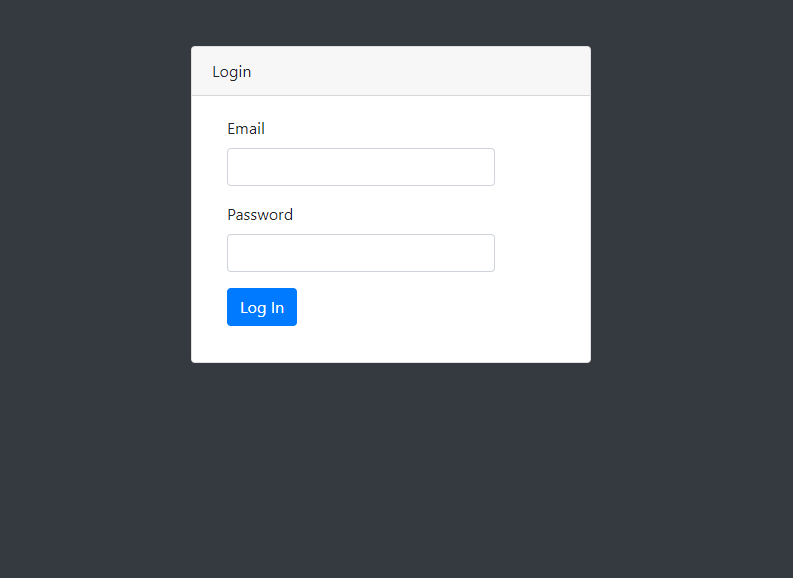
\includegraphics[width=\textwidth,keepaspectratio]{LogIn}
	\label{fig:LogIn}
\end{figure}
Pentru a putea folosi aplica\c tia, utilizatorul trebuie s\u a se autentifice.Dac\u a acesta \^incerc\u a s\u a intre pe o pagin\u a a site-ului
de administrare f\u ar\u a s\u a fie atuentificat, va fi redirec\c tionat c\u atre pagina de autentificare\ref{fig:LogIn}.Autentificarea se face prin 
intermediul adresei de email \c si o parol\u a.Un utilizator nu \^i\c si poate crea un cont nou deoarece,serviciul 
de \^inregistrare nu este un serviciu public,acesta destinat utiliz\u arii \^in cadrul unei companii, doar de 
persoane autorizate.Din acest punct de vedere, serviciul este similar cu o re\c tea intranet.
Pentru comfortul utilizatorului, am ales s\u a folosesc pentru autentificare cookie-uri a\c sa \^inc\^at
utilizatorul s\u a nu fie nevoit s\u a se autentifice de fiecare dat\u a c\^and dore\c ste s\u a intre \^in
aplica\c tie.Termenul de expirare al cookie-ului am decis s\u a fie 30 de minute.Cookie-ul este creat imediat dup\u a ce 
utilizatorul s-a atuentificat cu succes.

Mecanismul de autorizare din ASP.NET se bazeaz\u a pe atributul AuthorizeAttribute . Acesta se poate aplica unei metode
sau unui controller, caz \^in care va afecta toate metodele acestuia.Defapt exist\u a dou\u a atribute AuthorizeAttribute ,
unul pentru ASP.NET MVC \c si unul pentru Web Api.Diferen\c tele \^intre ele sunt destul de mici \c si din punct de vedere al utiliz\u arii
sunt identice.Aceste atribute se folosesc de o interfa\c t\u a numit\u a IPrincipal\ref{lst:IPrincipal}, care reprezint\u a utilizatorul.Am creat o interfa\c t\u a nou\u a care mo\c stene\c ste 
interfa\c ta IPrincipal, care s\u a \^imi ofere o metod\u a de a accesa rolurile utilizatorului.Implementarea noii interfe\c te implementeaz\u a
\c si interfa\c ta IPrincipal, deci poate fi folosit\u a pentru autorizare de c\u atre atributul AuthorizeAttribute.Pentru 
controllerele de Web APi pot folosi AuthorizeAttribute  \c si nu mai este nevoie s\u a fac o clas\u a derivat\u a a acestuia.
Pentru controllerele ASP.NET MVC,deoarece atributul este diferit de\c si se numes\c te la fel ca cel din Web Api, am ales s\u a
fac un nou atribut care s\u a mo\c steneasc\u a AuthorizeAttribute.Noul atribut \c stie s\u a trateze situa\c tiile 
\^in care utilizatorul nu este autorizat \c si s\u a \^il redirec\c tioneze pe acesta c\u atre o pagin\u a potrivit\u a situa\c tiei \^in 
care se afl\u a.Dac\u a utilizatorul nu este autentificat, atunci va fi redirec\c tionat c\u atre pagina de autentificare.Dac\u a 
este autentificat dar nu ar permisiunea necesar\u a acces\u arii pagini respective va fi redirec\c tionat c\u atre o pagin\u a de eroare 
corespunz\u atoare.

\^In momentul \^in care un utilizator se \^incearc\u a s\u a se autentifice,din motive de securitate,se calculeaz\u a o valoare hash a parolei
introduse.Apoi se caut\u a un cont \^in baza de date cu acela\c i email ca cel introdus de utilizator, dac\u a un asemenea cont este g\u asit,
se compar\u a hash-ul nou cu hash-ul salvat \^in baza de date.Dac\u a \^in urma compara\c tia,se decide c\u a parola utilizatorului este gre\c sit\u a,el
va fi \^intros c\u atre pagina de autentificare.Dac\u a parola introdus\u a este corect\u a se creaz\u a un principal de care este criptat \c si 
introdus \^intr-un cookie.Dup\u a ce este setat\u a durata p\^an\u a la expirarea cookie-ului, acesta este trimis c\u atre utilizator.

Pentru ca atributele de autorizare s\u a aib\u a un IPrincipal corect, acesta trebuie extras din cookie



\begin{lstlisting}[caption={Interfa\c ta IPrincipal},label={lst:IPrincipal},breaklines]
    //
    // Summary:
    //     Defines the basic functionality of a principal object.
    [ComVisible(true)]
    public interface IPrincipal
    {
        //
        // Summary:
        //     Gets the identity of the current principal.
        //
        // Returns:
        //     The System.Security.Principal.IIdentity object associated with the current principal.
        IIdentity Identity { get; }

        //
        // Summary:
        //     Determines whether the current principal belongs to the specified role.
        //
        // Parameters:
        //   role:
        //     The name of the role for which to check membership.
        //
        // Returns:
        //     true if the current principal is a member of the specified role; otherwise, false.
        bool IsInRole(string role);
    }
\end{lstlisting}

\section{Testare}

\section{Error Handling}

\section{Componente}

\subsection{NuGet}

NuGet est un manager de pachete gratuit \c si open-source creat pentru platforma .NET.Acesta a fost creat \^in 2010
\c si de atunci a devenit din ce \^in ce mai popular.Datorit\u a u\c surin\c tei cu care se pot aduce \^in proiect 
pachete externe, \c si posibilit\u a\c ti de publicare a acelor pachete, NuGet a devenit omniprezent \^in 
dezvoltarea aplica\c tiilor \^in cadrul platformei .NET.NuGet faciliteaz\u a dezvolatrea at\^at .NET Framework
c\^at \c si \^in .NET Core.NuGet este \c si mecanismul de \^imp\u ar\c tit cod sprijinit de Microsoft.
NuGet este distribuit ca o extensie de Visual Studio care \^incep\^and cu Visual Studio 2012 vine preinstalat\u a
\^in IDE.Popularitatea NuGet a condus la integrarea sa complet\u a \^in Visual Studio,\^in Visual Studio 2017 pe 
l\^ang\u a managementul pachetelor, NuGet poate fi folosit direct din IDE pentru \^impachetarea bibliotecilor
de clase.

%cum se face 
% ce bine e integrat
%un pachet e un zip
\^In dezvoltarea aplica\c tiilor din .Net, exist\u a o unealt\u a de management al depende\c telor externe numit NuGet.Acesta 
a fost dezvoltat de c\u atre 

\chapter{Utilizare}



\chapter{Planuri de viitor}

Add-Inuri cu javascript
Testare mai multa

\printbibliography

\end{document}

idei:
bootstrap
HTML
css
jquery
autofac
ce e un cookie